\documentclass[12pt,a4paper]{article}
\usepackage[utf8]{inputenc}
\usepackage[english]{babel}
\usepackage[T1]{fontenc}
\usepackage{amsmath}
\usepackage{amsfonts}
\usepackage{amssymb}
\usepackage{graphicx}
\usepackage{siunitx}
\usepackage{float}
\usepackage[left=2cm,right=2cm,top=2cm,bottom=2cm]{geometry}
\author{Gerald}
\bibliographystyle{plain}

\begin{document}
\sisetup{separate-uncertainty = true}
	\setlength{\parindent}{0pt} 
	\begin{center}
		{\LARGE Experiment protocol}\\
		\begin{large}
			for the solid state lab course\\[0.4cm]
			at RWTH Aachen\\
			II. Physikalisches Institut A\\[5.5cm]
			\Large\textbf{\textsl{Raman characterization of CVD grown graphene}}\\[5.5cm]
			\normalsize\textit{authored\\by}\\[0.4cm]
			\large{Moritz Berger (355244)\\Gerald Kolter (355005)}\\[2cm]
			\large \textbf{Summer term 2019}
		\end{large}
	\end{center}
	\newpage
	
	\tableofcontents
	\newpage

\section{Introduction}
Novoselov et al. were the first to intentionally isolate a mono-layer of carbon atoms from a graphit block, called graphene.\cite{Novoselov2004} Since then it attracted an overwhelming interest in fundamental and applied research in a variety of fields, such as solid state physics, electronics, mechanics, and optics.\cite{NeumannStampfer} \\
Confocal Raman Spectroscopy provides the ability to obtain important material characteristics locally and noninvasively.\cite{NeumannStampfer} \\
Figure \ref{fig:Exfoliation_Spectra} shows a Raman spectra analyzed later. One can mainly see three peaks. The high peak at about \SI{1600}{\per cm} is called the "G" peak, the lower peak at about \SI{2700}{\per cm} is called "2D" peak and the lowest peak at about \SI{2400}{\per cm} is called "D+D''" peak. The positions of the peak are denoted by $\omega _G$, $\omega _{2D}$ and $\omega _{D+D''}$ and the Full Width at Half Maximum (FWHM) are denoted by $\Gamma _G$, $\Gamma _{2D}$ and $\Gamma _{D+D''}$ respectively. \\
The G peak originates from the highest optical phonons at the $\Gamma$ point in the lattice. The 2D peak originates from the breathing mode of the TO branch around the K point in the lattice. The D+D'' originates from defects.\cite{NeumannStampfer}


\section{Analysis of the single spectra}
Over the course of this report single Raman spectra have to be analyzed. This chapter explains the method used to extract the relevant values of the Raman peaks.\\
An example of a spectrum is shown in figure \ref{fig:example_spectrum}. There are two peaks visible in this spectrum. A Lorentz-curve of the form
\begin{equation}
f(\omega) = a + b \cdot x + \dfrac{c \gamma}{(\omega^2-\omega_0^2)^2 + \gamma^2}
\label{eq:fit}
\end{equation}
is fitted to a small area that fully includes the peak. $\omega_0$ denotes the peak position. Its error follows directly from the fit. The linear part in equation \ref{eq:fit} is necessary, because some of the spectra show a strong background noise, which makes it hard to extract the peak intensity, which is necessary for the calculation of the FWHM. The background noise is assumed to be a linear function in the fitting area.\\
In order to extract the FWHM this linear part is subtracted from the fit and the two points of the fit which are at half of the peak maximum are determined. The distance of these points give us the FWHM. The error of this value is determined by propagating the error of the fit.
\begin{figure}
\centering
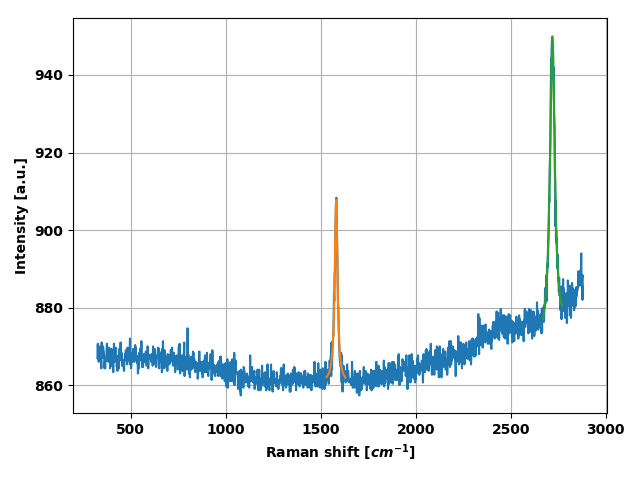
\includegraphics[scale=0.5]{Bilder/part6/1.png}
\caption{Example of the measured Raman spectrum of graphene. The Lorentz-curve fits against the two visible peaks are also shown.}
\label{fig:example_spectrum}
\end{figure}

\section{Exfoliation}
Exfoliation is the simplest technique to isolate graphene from a graphit block.

\subsection{Method}
In order to isolate a mono-layer of carbon atoms with exfoliation one uses a sticky tape and a graphit block. The first step is to place the graphit onto the sticky tape and pull it off again. After this one can see a film of graphit on the sticky tape. The second step is to press a sticky tape on the graphit film and pull it off again. This second step is repeated until one gets a mono-layer of carbon atoms.

\subsection{Results}

\begin{figure}
\centering
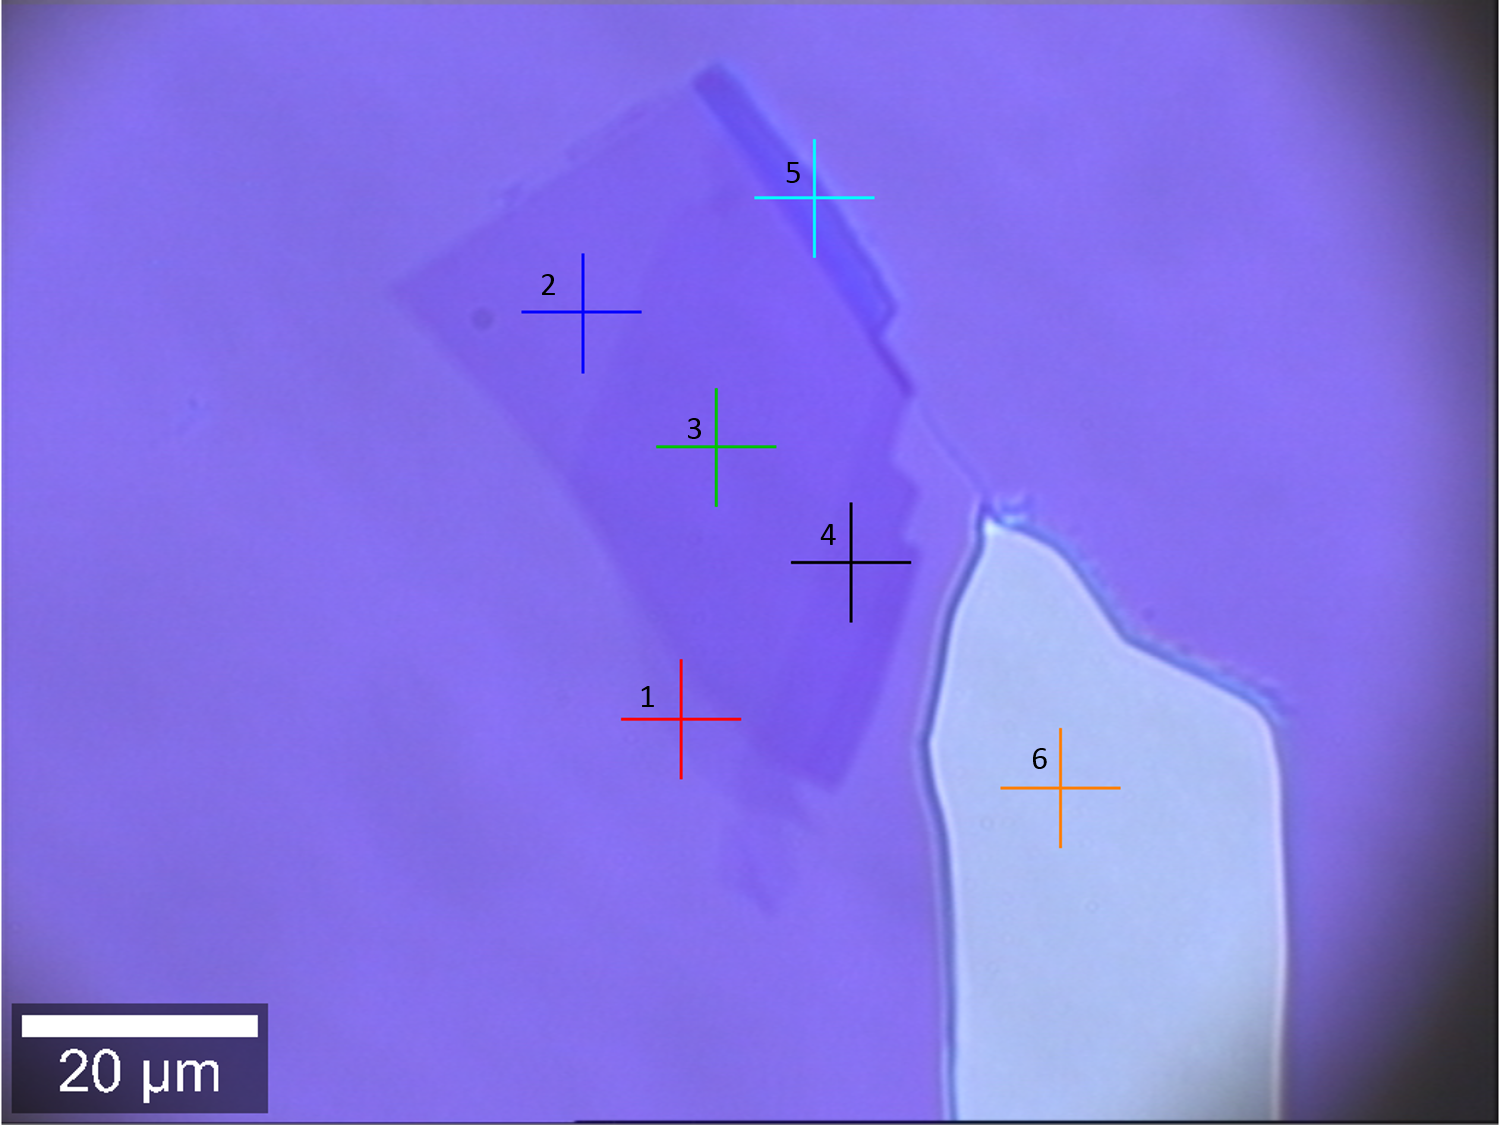
\includegraphics[scale=0.35]{Bilder/Exfoliation/mono_bi_tri_flake.PNG}
\caption{Image from one flake of graphene isolated by Exfoliation made with an optical microscope. The crosses mark the points where the Raman spectra are extracted.}
\label{fig:Exfoliation_Microscope}
\end{figure}

Figure \ref{fig:Exfoliation_Microscope} shows one of the flakes obtained by Exfoliation made with an optical microscope. This flake shows different numbers of layer in different areas. The higher the contrast the higher the number of layer. In the right upper area the flake is most likely to consist of a single layer of carbon atoms. The left lower area is presumably two layer of carbon atoms and the other are like stairs, each one layer of carbon atoms more.

\begin{figure}
\centering
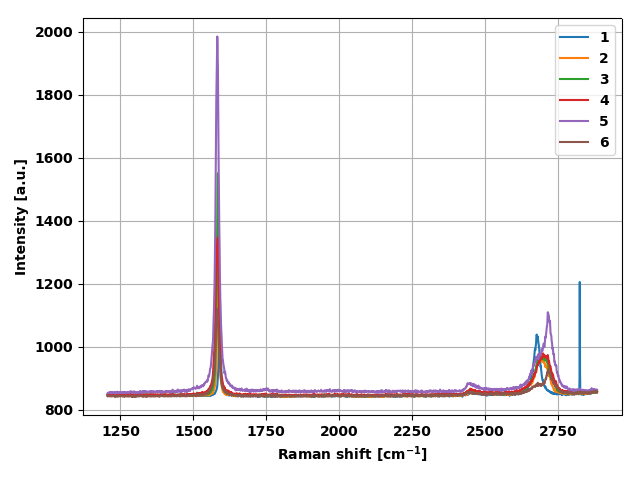
\includegraphics[scale=0.5]{Bilder/Exfoliation/2_mono_bi_tri_flake_all.PNG}
\caption{Raman spectra from the flake shown in Fig. \ref{fig:Exfoliation_Microscope}.}
\label{fig:Exfoliation_Spectra}
\end{figure}

\begin{figure}
\centering
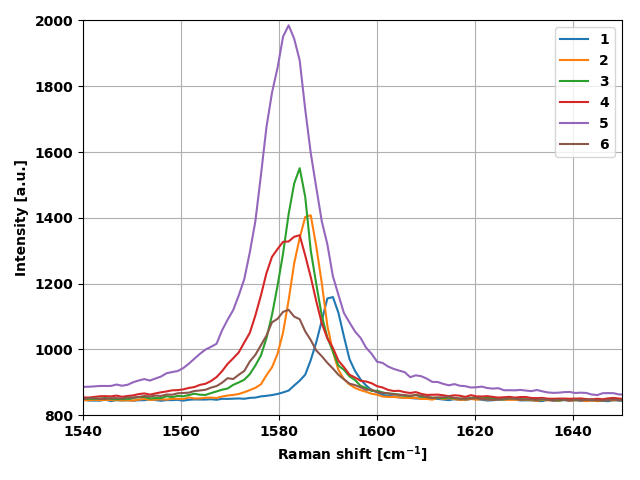
\includegraphics[scale=0.5]{Bilder/Exfoliation/2_mono_bi_tri_flake_G_peaks.PNG}
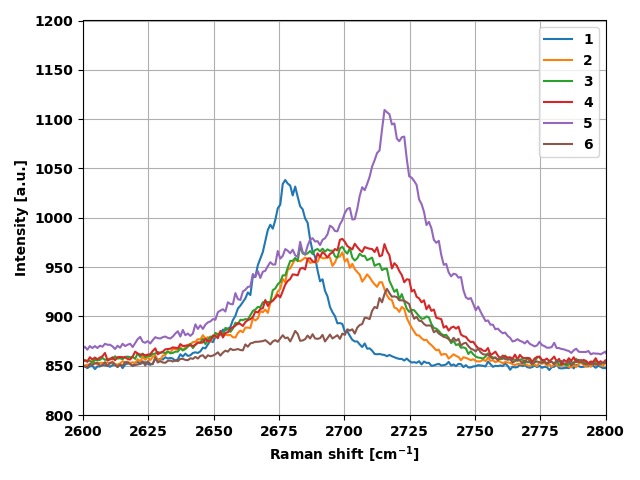
\includegraphics[scale=0.5]{Bilder/Exfoliation/2_mono_bi_tri_flake_2D_peaks.PNG}
\caption{\textbf{Left} G-Peak and \textbf{Right} 2D-Peak of the Raman spectra from the flake shown in Fig. \ref{fig:Exfoliation_Microscope}.}
\label{fig:Exfoliation_Peaks}
\end{figure}

\begin{table}[h]
\centering
\begin{tabular}{|c|c|c|}
\hline 
Measurement point & I(G) [a.u.] & suggested number of layers \\ 
\hline 
1 & 1159.0 & 1 \\ 
\hline 
2 & 1407.7 & 2-3 \\ 
\hline 
3 & 1551.0 & 3-4 \\ 
\hline 
4 & 1347.0 & 2 \\ 
\hline 
5 & 1985.3 & >5 \\
\hline 
6 & 1120.3 & -  \\ 
\hline 
\end{tabular} 
\caption{Results for the positions and width of G and 2D peak from the spectra at the measurement points as marked in Fig. \ref{fig:Part2_map_microscope}.}
\label{tab:step_G_intensities}
\end{table}

Figure \ref{fig:Exfoliation_Spectra} shows the Raman spectra at the measurement points as shown in figure \ref{fig:Exfoliation_Microscope}. \\
The integrated intensity of the G line increases linearly with the number of layers. For more than five layers the intensity starts to saturate to the bulk value. The 2D peak also depends on the number of layers. This time the shape variies. For highly orientated pyrolytic graphite (HOPG) it is composed of two Lorentzian contributions, for doublelayer graphene four subpeaks can be assigned, for the singlelayer only one Lorentzian peak is left \cite{Lett_2007}. \\
With this knowledge one can see, that the area at measurement point 1 a single layer of carbon atoms is, as the 2D-peak (Fig. \ref{fig:Exfoliation_Peaks}) is a sharp single Lorentzian. The measured intensities of the G-peaks would suggest that the number of layers at the measurement point 4 is lower than at the measurement point 2 and 3. Which is surprising because the contrast in the micrscope image of the flake (Fig. \ref{fig:Exfoliation_Microscope}) would suggest it the other way around. \\
At the measurement point 6 the G-peak intensity is dropped even below the intensity of the single layer. At this position the flake looks different even in the microscope image (Fig. \ref{fig:Exfoliation_Microscope}). It can only be guessed what is happening at this point.



\section{Gr flake with wrinkle}

\begin{figure}
\centering
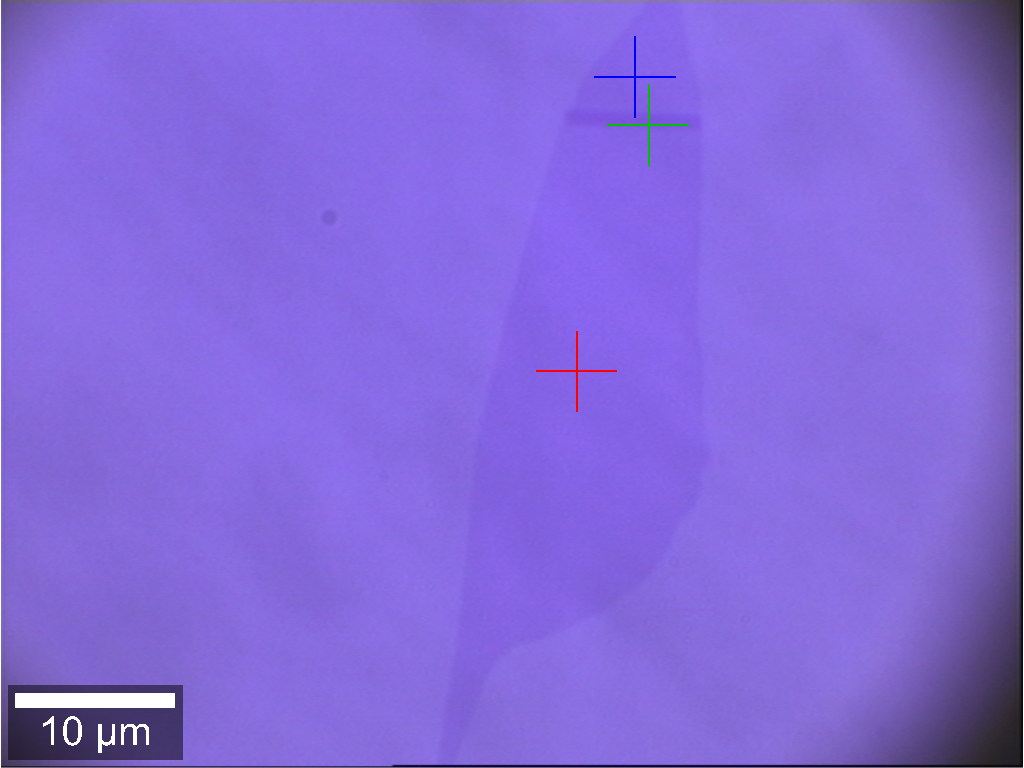
\includegraphics[scale=0.3]{Bilder/Wrinkle/mono_single_spectra.PNG}
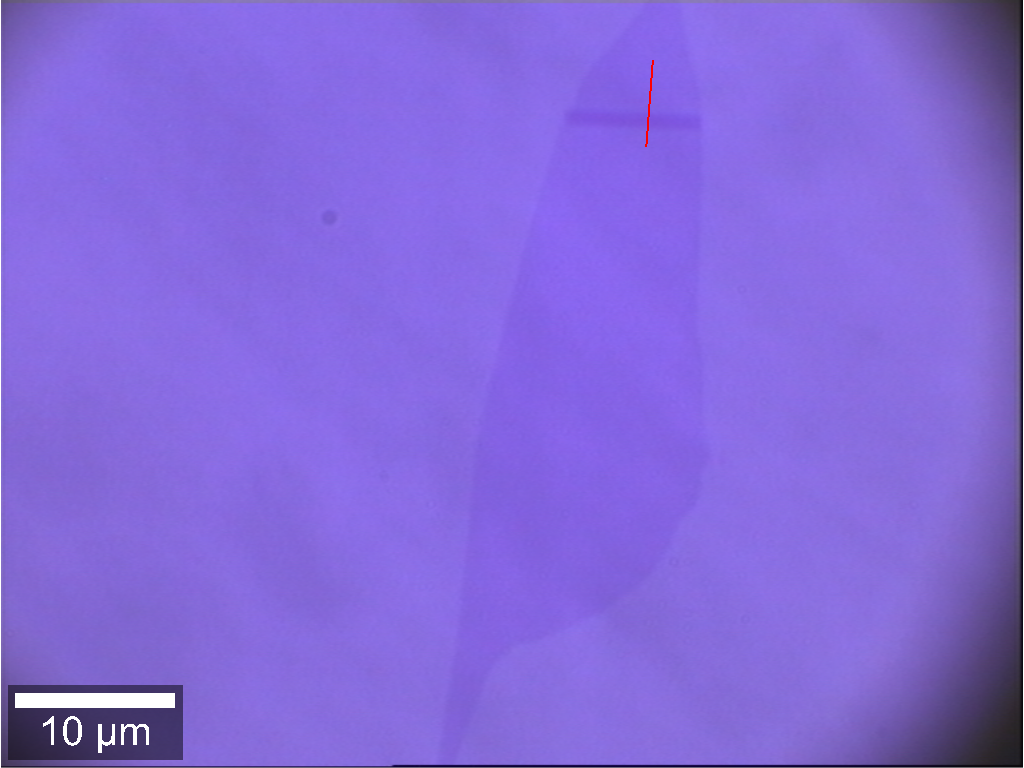
\includegraphics[scale=0.22]{Bilder/Wrinkle/mono_line_scan.PNG}
\caption{Microscope image from one graphene flake that showed an interesting wrinkling feature. \textbf{Left}: The crosses mark the points where the single Raman spectra are extracted. \textbf{Right}: Also a line scan were performed.}
\label{fig:wrinkle_microscope}
\end{figure}

One of the Gr flakes produced by Exfoliation showed an interesting feature. A small part of the flake has a higher contrast in the microscope image than the rest (Fig. \ref{fig:wrinkle_microscope}).


\subsection{Single spectra}

\begin{figure}
\centering
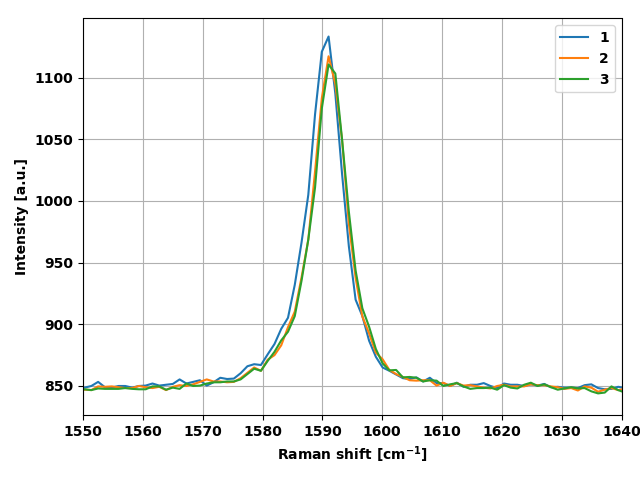
\includegraphics[scale=0.5]{Bilder/Wrinkle/single_spectra/single_spectra_G_peak.PNG}
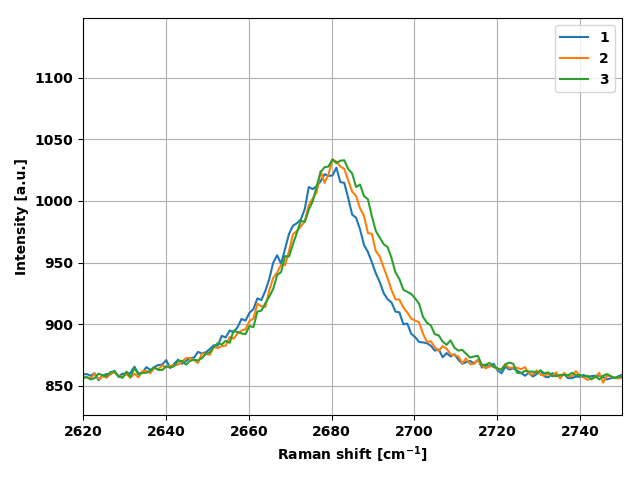
\includegraphics[scale=0.5]{Bilder/Wrinkle/single_spectra/single_spectra_2D_peak.PNG}
\caption{\textbf{Left} G-Peak and \textbf{Right} 2D-Peak of the Raman spectra from the flake shown in Fig. \ref{fig:wrinkle_microscope} on the left.}
\label{fig:wrinkle_Peaks}
\end{figure}

\begin{table}[h]
\centering
\begin{tabular}{|c|c|}
\hline 
I(G) & 1133.3 a.u. \\ 
\hline 
$\omega _G$ & \SI{1589.95}{\per cm} \\ 
\hline 
$\Gamma _G$ & \SI{4.96}{\per cm} \\ 
\hline 
$\omega _{2D}$ & \SI{2678.22}{\per cm} \\ 
\hline 
$\Gamma _{2D}$ & \SI{23.14}{\per cm} \\ 
\hline 
\end{tabular} 
\caption{Results for the single spectra as shown in Fig. \ref{fig:wrinkle_Peaks}. The three measurement showed identical results, therefor its only one result presented here.}
\label{tab:wrinkle_single_results}
\end{table}

As one can see in Fig. \ref{fig:wrinkle_Peaks} the G and 2D peaks are in all 3 single spectrum measurements identical. Presumably the measurement point 3 was to low and therefor is in the same area as measurement point 1. \\
However the measured values (see table \ref{tab:wrinkle_single_results}) suggest a mono layer at both sides of the feature. The feature itself has to be analyzed with the line scan as done in the next chapter.


\subsection{Line scan}

\begin{figure}
\centering
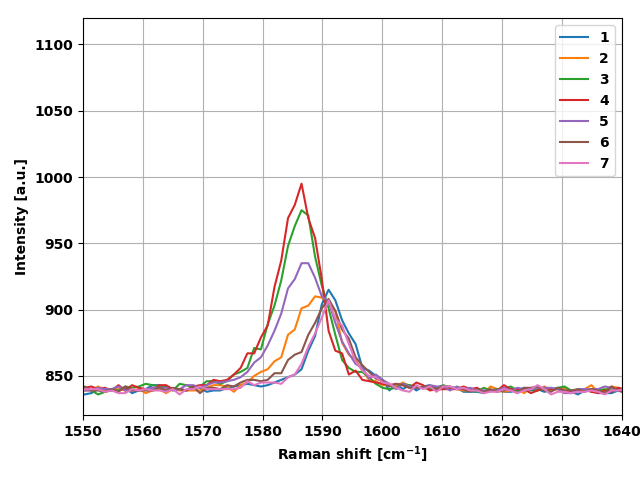
\includegraphics[scale=0.5]{Bilder/Wrinkle/line_scan/line_scan_G_peak.PNG}
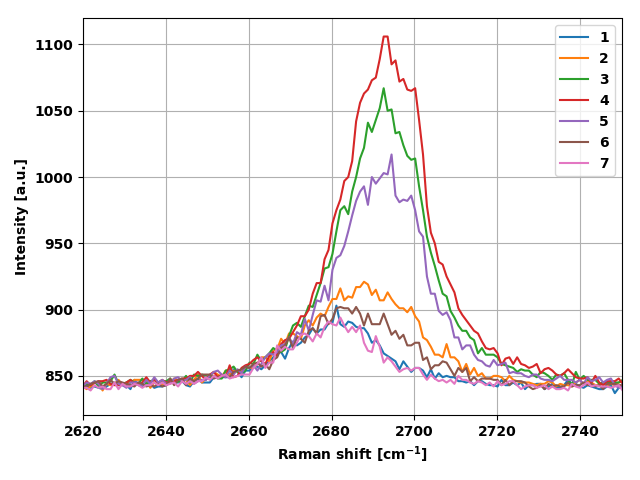
\includegraphics[scale=0.5]{Bilder/Wrinkle/line_scan/line_scan_2D_peak.PNG}
\caption{\textbf{Left} G-Peak and \textbf{Right} 2D-Peak of the Raman spectra from the flake shown in Fig. \ref{fig:wrinkle_microscope} (right) measured with a line scan.}
\label{fig:wrinkle_line_Peaks}
\end{figure}

The line scan performed seven single spectrum measurement equally contributed over the red line as marked in Fig. \ref{fig:wrinkle_microscope} on the right. The measured G and 2D peaks are shown in Fig. \ref{fig:wrinkle_line_Peaks}. \\
As one can see both peaks are identical for the first and the last two measurement. This suggests, that measurements 3, 4 and 5 are on the feature. As the G-peak of measurement 5 is significantly smaller than those from measurement 3 and 4 one suspects, that measurement 5 is on the border of the feature. Therefor in the following only measurement 3 and 4 are used.



\section{Half Sandwich on PMMA}
A graphene flake is placed on a hexagonal boron nitride (hBN) film, which is applied on a Polymethylmethacrylat (PMMA) sample. 

\subsection{Single Spectra}

\begin{figure}
\centering
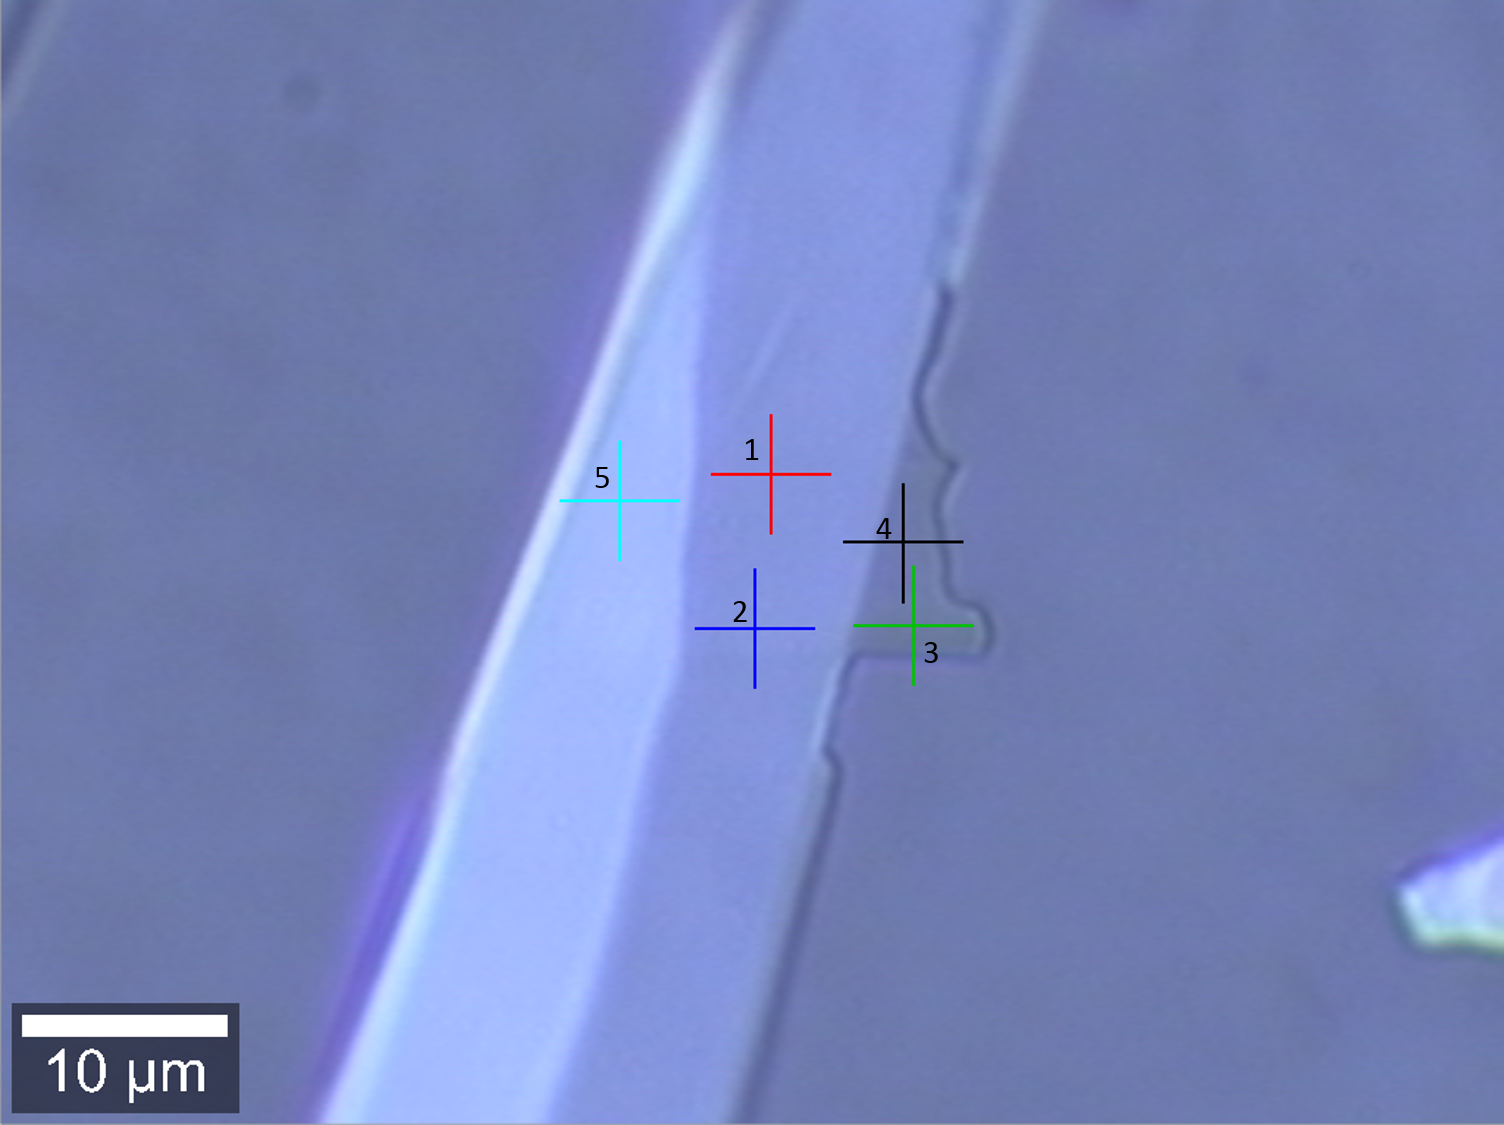
\includegraphics[scale=0.25]{Bilder/Part_2/4_Half_sandwich_on_PMMA.PNG}
\caption{Image from one graphene hBn sandwich made with an optical microscope. The crosses mark the points where the Raman spectra are extracted.}
\label{fig:Part2_map_microscope}
\end{figure}

\begin{table}[h]
\centering
\begin{tabular}{|c|c|c|c|c|}
\hline 
Measurement & $\omega _G$ & $\Gamma _G$ & $\omega _{2D}$ & $\Gamma _{2D}$ \\ 
point &  &  &  &  \\ 
\hline 
1 & \SI{1584.25 \pm 0.15}{\per cm} & \SI{12.57 \pm 0.25}{\per cm} & \SI{2680.89 \pm 0.16}{\per cm} & \SI{17.19 \pm 0.52}{\per cm} \\ 
\hline 
2 & \SI{1582.95 \pm 0.16}{\per cm} & \SI{11.59 \pm 0.13}{\per cm} & \SI{2695.50 \pm 0.35}{\per cm} & \SI{50.37 \pm 0.49}{\per cm} \\ 
\hline 
3 & \SI{1582.44 \pm 0.17}{\per cm} & \SI{13.68 \pm 0.11}{\per cm} & \SI{2694.61 \pm 0.27}{\per cm} & \SI{52.02 \pm 0.36}{\per cm} \\ 
\hline 
4 & \SI{1583.30 \pm 0.55}{\per cm} & \SI{16.26 \pm 0.10}{\per cm} & \SI{2693.79 \pm 0.29}{\per cm} & \SI{35.06 \pm 0.43}{\per cm} \\ 
\hline 
5 & \SI{1583.32 \pm 0.21}{\per cm} & \SI{12.31 \pm 0.25}{\per cm} & \SI{2692.23 \pm 0.16}{\per cm} & \SI{13.09 \pm 0.23}{\per cm} \\ 
\hline 
\end{tabular} 
\caption{Results for the positions and width of G and 2D peak from the spectra at the measurement points as marked in Fig. \ref{fig:Part2_map_microscope}.}
\label{tab:Sandwich_Results}
\end{table}

Table \ref{tab:Sandwich_Results} shows the measured positions and width of the G and 2D peak at every measurement point as marked in figure \ref{fig:Part2_map_microscope}. \\
As one can see the position of the G peak differs only a little bit. The width of the G peak sway around approximately 20\%. \\
The magnitude of the variation of the 2D peak position is similar to the one from the G peak. The width of the G peak is variing a lot more than the one of the 2D peak.


\subsection{$\Gamma _{2D}$ map}

\begin{figure}
\centering
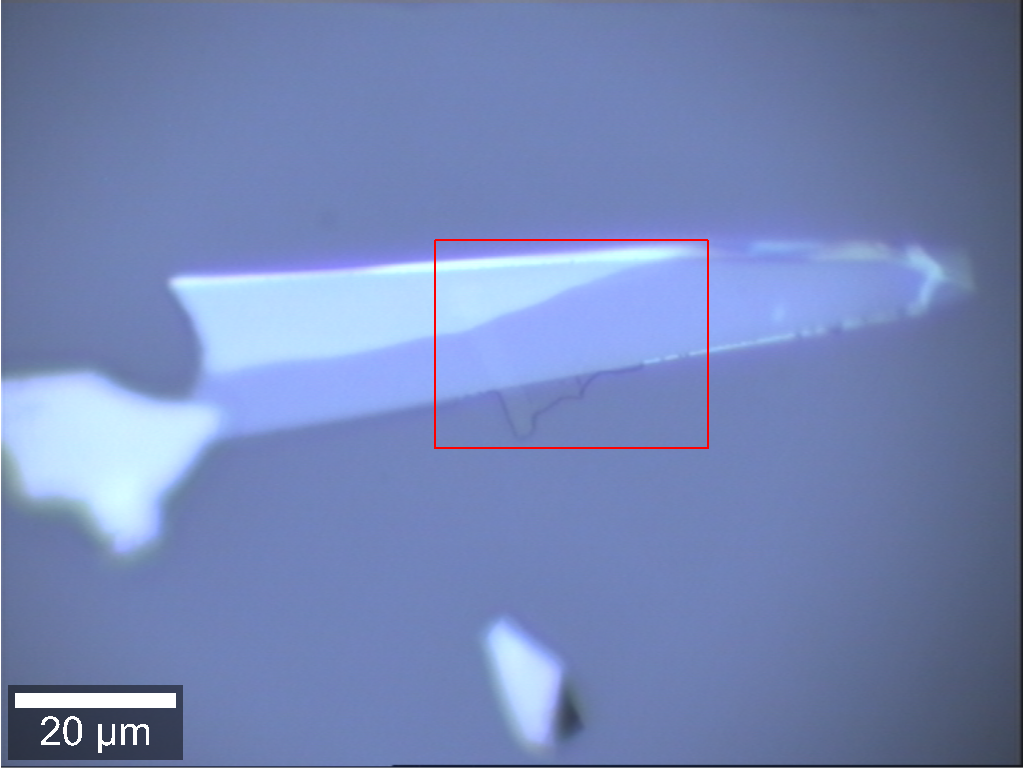
\includegraphics[scale=0.2]{Bilder/Part_2/half_sandwich_map.PNG}
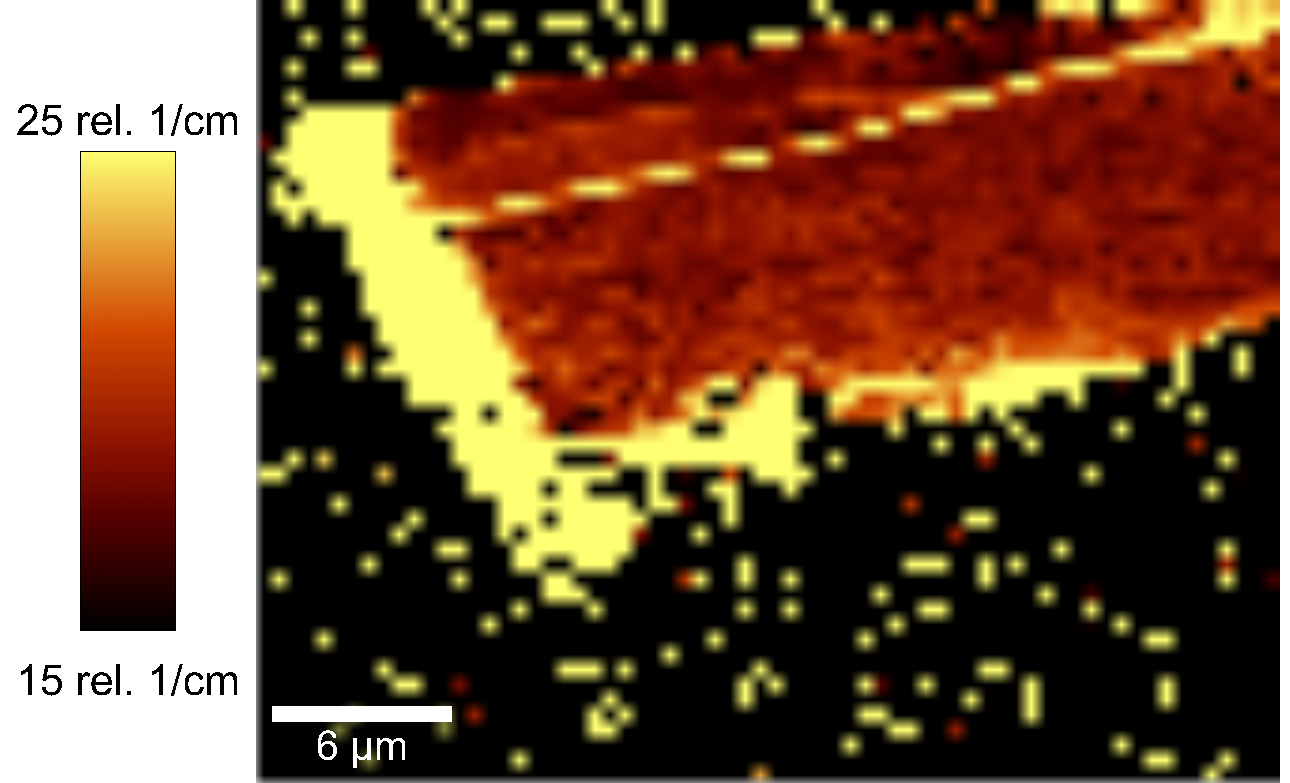
\includegraphics[scale=0.2]{Bilder/Part_2/half_sandwich_map_2D_width.PNG}
\caption{The upper image shows the microscope image of the flake. The lower image shows the map of $\Gamma _{2D}$ from the red boxed part.}
\label{fig:Part2_map}
\end{figure}

Figure \ref{fig:Part2_map} shows a $\Gamma _{2D}$ map of the same flake as analyzed with the five single spectra before. \\
On the map one can see a superposition of the structure of the graphene flake and the structure of the hBn. Those areas on which graphene and hBn are present are colored red which corresponds to a $\Gamma _{2D}$ of around \SI{20}{\per cm}. Where neither of those are present the color is black which corresponds to a $\Gamma _{2D}$ of around \SI{15}{\per cm}. The edges of the graphene flake are colored yellow which corresponds to a $\Gamma _{2D}$ of around \SI{25}{\per cm}.



\section{Combining Analysis}
From the analyzed spectra one gets each $\omega _G$, $\omega _{2D}$, $\Gamma _G$ and $\Gamma _{2D}$. With all these values one can plot $\omega _G$ vs. $\omega _{2D}$ and $\Gamma _G$ vs. $\Gamma _{2D}$. These provide the possibility for further analysis.


\subsection{$\omega _G$ vs. $\omega _{2D}$}


\begin{table}[h]
\centering
\begin{tabular}{|c|c|c|}
\hline 
Measurement & strain [\%] & doping [\SI{E12}{\per c \cubic m}] \\ 
point &  & \\ 
\hline 
1 & 0.203 & 4.950 \\
\hline 
2 & 0.638 & 0.028 \\
\hline 
3 & 0.701 & 0.637 \\
\hline 
4 & 0.845 & 3.017 \\
\hline 
5 & 1.218 & 6.020 \\
\hline 
6 & 1.328 & 7.804 \\
\hline 
\end{tabular} 
\caption{Strain and doping of the stair flake as shown in Fig. \ref{fig:Exfoliation_Microscope} calculated with vector decomposition.}
\label{tab:step_strain_doping}
\end{table}

\begin{table}[h]
\centering
\begin{tabular}{|c|c|c|}
\hline 
Measurement & strain [\%] & doping [\SI{E12}{\per c \cubic m}] \\ 
point &  & \\ 
\hline 
1 & 0.212 & 4.314 \\
\hline
2 & 0.284 & 4.440 \\
\hline
3 & 0.339 & 4.279 \\
\hline 
\end{tabular} 
\caption{Strain and doping of the mono layer flake calculated with vector decomposition.}
\label{tab:wrinkle_strain_doping}
\end{table}

\begin{table}[h]
\centering
\begin{tabular}{|c|c|c|}
\hline 
Measurement & strain [\%] & doping [\SI{E12}{\per c \cubic m}] \\ 
point &  & \\ 
\hline 
1 & 0.192 & 0.157 \\
\hline
2 & 0.675 & 1.030 \\
\hline
3 & 0.634 & 1.168 \\
\hline
4 & 0.623 & 0.639 \\
\hline
5 & 0.568 & 0.459 \\
\hline 
\end{tabular} 
\caption{Strain and doping of the half sandwich on PMMA as shown in Fig. \ref{fig:Part2_map_microscope} calculated with vector decomposition.}
\label{tab:PMMA_strain_doping}
\end{table}


\begin{figure}
\centering
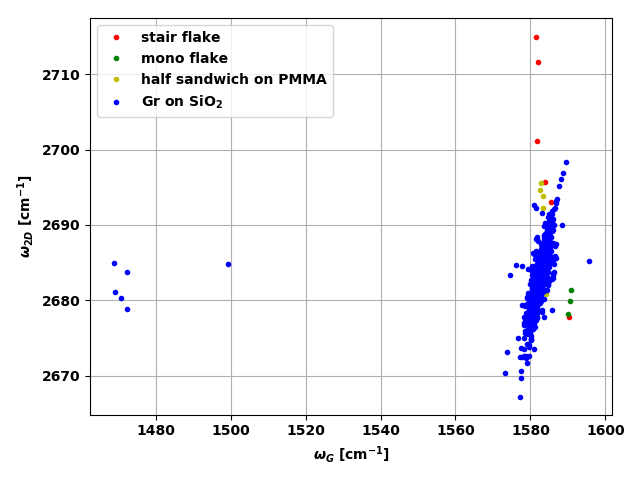
\includegraphics[scale=0.55]{Bilder/Part_3/omega_2D_vs_G.PNG}
\caption{$\omega _G$ vs. $\omega _{2D}$ for the measurements of the stair flake as shown in Fig. \ref{fig:Exfoliation_Microscope}, a monolayer flake, the half sandwich on PMMA as shown in Fig. \ref{fig:Part2_map_microscope} and a graphene flake on SiO$_2$ as analyzed later.}
\label{fig:Part3_omega_G_vs_2D}
\end{figure}

Fig. \ref{fig:Part3_omega_G_vs_2D} shows all measured values for $\omega _G$ and $\omega _{2D}$ plotted. \\
As one can see, apart from a few measured points for the graphene on SiO$_2$ the points are pretty close to each other. Especially if one takes into account, that the measurements for the graphene on SiO$_2$ which come from a map measurement of the same sample are widely spread. \\
The spreading in this plot originates from the strain and doping. Strain induces a relative shift along a straight line with slope 2.2, while doping a shift along a straight line with slope 0.7 induces \cite{NeumannStampfer}. The intersection of these two lines is at $\omega _{\text{G, prestine}}$ and $\omega _{\text{2D, prestine}}$ which are the values for prestine graphene and are given as: 
\begin{equation*}
\omega _{\text{G, prestine}} = \SI{1581.6}{\per cm} \quad \text{and} \quad \omega _{\text{2D, prestine}} = \SI{2676.9}{\per cm}
\end{equation*} \\

Tables \ref{tab:step_strain_doping}, \ref{tab:wrinkle_strain_doping} and \ref{tab:PMMA_strain_doping} show the results for the calculated strain and doping of the measurement points as plotted in Fig. \ref{fig:Part3_omega_G_vs_2D}.  For the graphene on SiO$_2$ there are too many points to display all calculated strain and doping. So at this point just the average strain and doping are stated:
\begin{equation*}
\bar{\epsilon} _{SiO_2} = 0.238 \, \% \qquad \bar{n} _{SiO_2} = \SI{2.610}{\per c \cubic m}
\end{equation*}


\subsection{$\Gamma _G$ vs. $\Gamma _{2D}$}


\begin{figure}
\centering
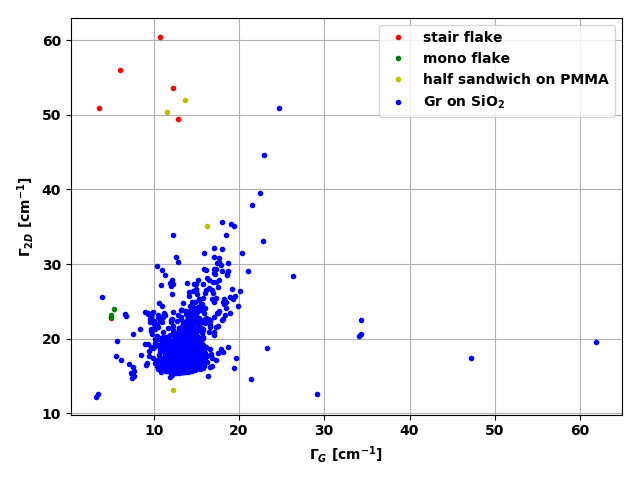
\includegraphics[scale=0.55]{Bilder/Part_3/gamma_2D_vs_G.PNG}
\caption{$\Gamma _G$ vs. $\Gamma _{2D}$ for the measurements of the stair flake as shown in Fig. \ref{fig:Exfoliation_Microscope}, a monolayer flake, the half sandwich on PMMA as shown in Fig. \ref{fig:Part2_map_microscope} and a graphene flake on SiO$_2$ as analyzed later.}
\label{fig:Part3_gamma_G_vs_2D}
\end{figure}

Fig. \ref{fig:Part3_gamma_G_vs_2D} shows all measured values for $\Gamma _G$ and $\Gamma _{2D}$ plotted. \\ 
As expected the graphene flake consisting of only one layer has a low $\Gamma _G \approx \SI{5}{\per cm}$ and a low $\Gamma _{2D} \approx \SI{23}{\per cm}$. \\
As one can see the graphene on SiO$_2$ has a low $\Gamma _{2D}$ and $\Gamma _G$ with a few points which has either a higher $\Gamma _{2D}$ or $\Gamma _G$. Actually no measurement resulted in a $\Gamma _{2D} > \SI{30}{\per cm}$ and $\Gamma _G > \SI{30}{\per cm}$. Interestingly the measurements for the stair flake and the sandwich on PMMA only have $\Gamma _{2D} > \SI{30}{\per cm}$, but still a $\Gamma _G < \SI{15}{\per cm}$.

\section{Impact of the Laser wavelength}
The encapsulated graphene is used to analyze the impact of the Laser wavelength on the Raman spectrum. The $\omega_g$ vs. $\omega_{2D}$ map and $\Gamma_g$ vs. $\Gamma_{2D}$map are shown in figure \ref{fig:Laser_omega} for both Lasers. The distribution of the individual positions are also shown in figure \ref{fig:Laser_omega_hist}.\\
The $\omega_g$ position is not shifted at all. However the $\omega_{2D}$ position shifted from an average position of \SI{2719(3)}{cm^{-1}} for the blue laser to \SI{2683(3)}{cm^{-1}} for the green laser. The reason for this is that only a single electron/hole site participates in the Raman process that leads to the G-line. By changing the Laser frequency only the excitation energy changes. The Raman shift stays the same. The 2D-line requires two lattice sites and the phonon modes connect them. Changing the excitation energy also changes the phonon modes and with that the Raman shift.\\
The higher energy of the blue laser also shifts the average FWHM, as seen in figure \ref{fig:Laser_gamma_hist}. $\Gamma_g$ is larger on average for the blue laser, while $\Gamma_{2D}$ is smaller compared to the green laser. In general the measurement taken with the blue laser seems to be broadly distributed. However this is most likely a consequence of different measurement settings.\\
\\

\begin{figure}
\centering
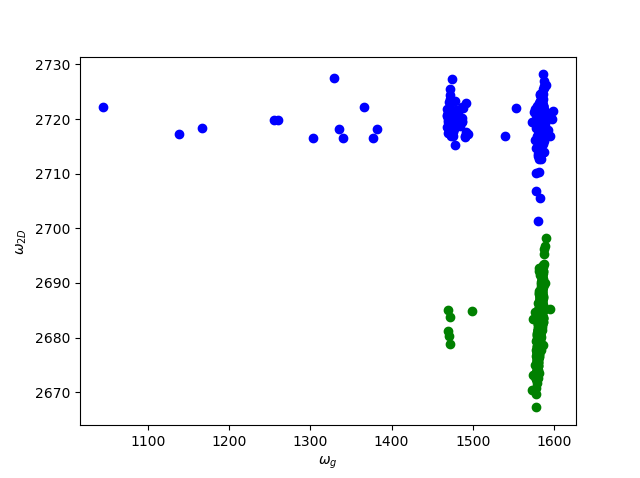
\includegraphics[scale=0.5]{Bilder/Laser/omega.png}
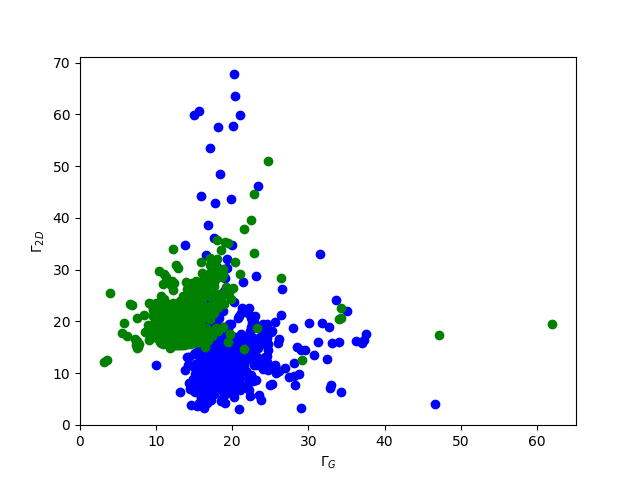
\includegraphics[scale=0.5]{Bilder/Laser/gamma.png}
\caption{line data of the G-line plotted against the 2D-line for both Lasers. Left: $\omega$, right: $\Gamma$. The Data point of the green laser are plotted in green and the blue laser in blue.}
\label{fig:Laser_omega}
\end{figure}

\begin{figure}
\centering
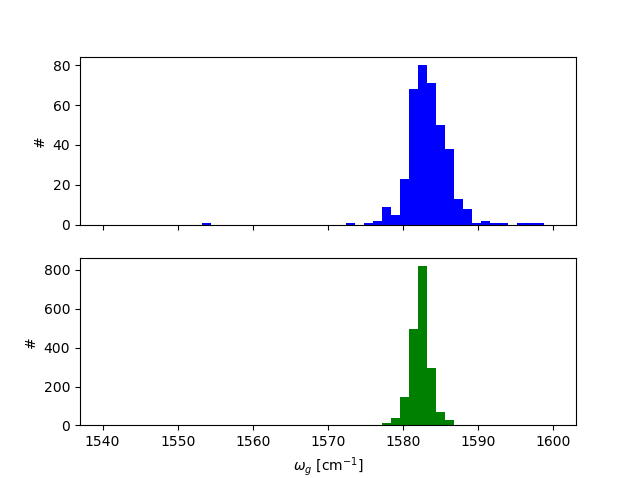
\includegraphics[scale=0.5]{Bilder/Laser/omegag_hist.png}
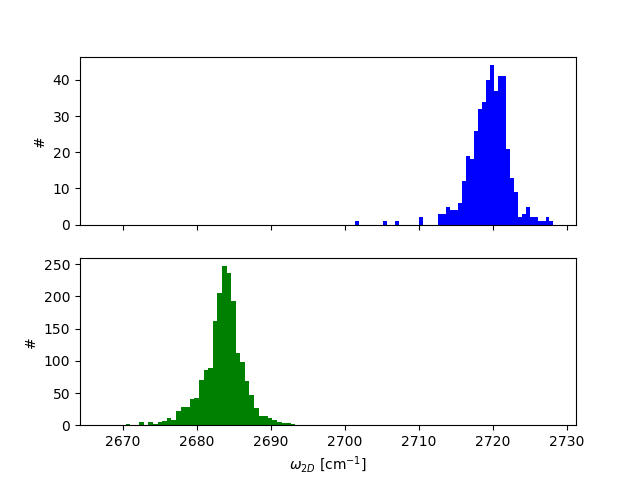
\includegraphics[scale=0.5]{Bilder/Laser/omega2d_hist.png}
\caption{Distribution of the line positions for the blue(top) and green(bottom) Laser. Right: $\omega_{g}$, left: $\omega_{2D}$.}
\label{fig:Laser_omega_hist}
\end{figure}

\begin{figure}
\centering
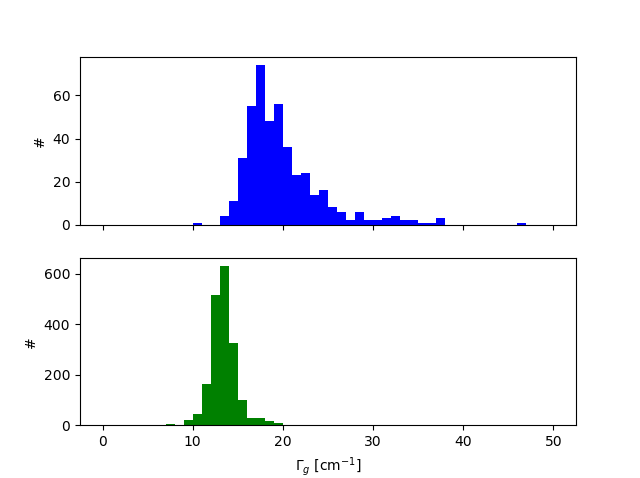
\includegraphics[scale=0.5]{Bilder/Laser/gammag_hist.png}
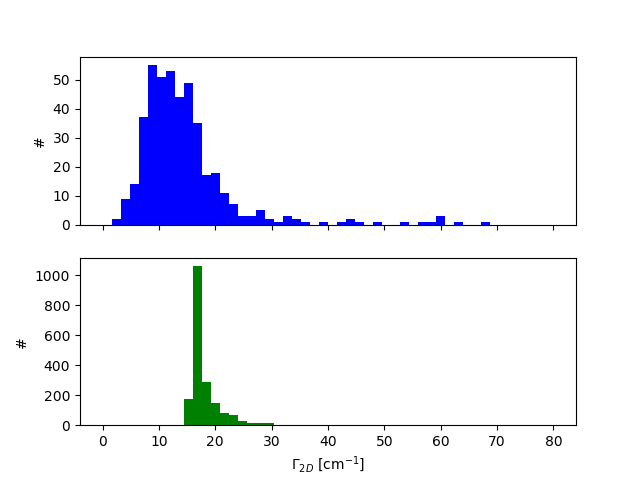
\includegraphics[scale=0.5]{Bilder/Laser/gamma2d_hist.png}
\caption{Distribution of the FWHD for the blue(top) and green(bottom) Laser. Right: $\Gamma_{g}$, left: $\Gamma_{2D}$.}
\label{fig:Laser_gamma_hist}
\end{figure}

\section{Polycrytalline Cu sample}
This sample is used to analyze the strain of CVD graphene on on a Cu-substrate for different lattice orientations. The Raman-measurement is done with the blue laser.\\ In a first step the $\omega_{g/2D}$ positions for pristine graphene when using this laser are determined and used as reference for the strain calculation. The spectrum of pristine graphene is shown in figure \ref{fig:pristine}. Both lines have a very low intensity, which indicates that there was no graphene at the point where the spectrum was taken. The 2D-line can be analyzed, which results in  $\omega_{2D} = \SI{2721.1(4)}{cm^{-1}}$. However the G-line intensity is too small to be analyzed. Based on the previous chapter we can assume that the G-line does not shift when changing the laser. This means the Raman of this line should be the same as in the spectrum of pristine graphene taken with the green laser, which is shown in figure \ref{fig:pristine_green}. The G-line frequency is $\omega_{G} = \SI{1582.4(3)}{cm^{-1}}$.\\
\\
The polycrystalline sample and the measurement points are shown in figure  \ref{fig:poly_sample} and the extracted line positions in table \ref{tab:part5_pos}. The point were taken on three different lattice orientations. \\
\\
erklärung analysis.........
\\
\\
The results are shown in table \ref{tab:part5_results}. The Measurement point 1, 3 and 6 were taken in an area where the visible oxidization was low. This is reflected in the low doping concentration at these point. Points 2 and 7 were expected to have a high oxidization, which is also reflected in the data.\\
Points 4 and 5 do not reflect the expectation. However it is possible that the sample was moved during measurement so that point 4 was measured at low oxidization and point 5 at high oxidization.\\
It should also be noted that the position of points 1 and 6 in the map in figure \ref{fig:poly_sample} is left of the strain-line. This technically results in negative doping and is most likely a consequence of an inaccurate measurement resulting in a systematical error, which is not analyzed.\\
\\
The strain is directly impacted by the oxidization. Areas with low doping also show low strain, whereas areas with high doping show high strain. In comparison to this the lattice orientation has a very small impact. Because of the potential systematical error it is impossible to determine the lattice orientation which gives the best result.

\begin{figure}
\centering
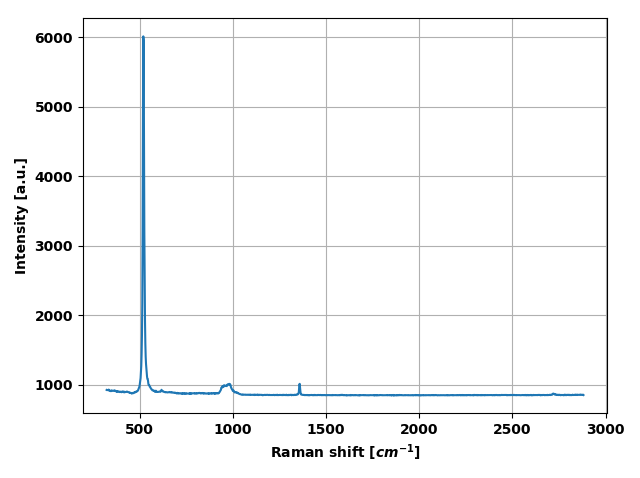
\includegraphics[scale=0.5]{Bilder/part6/prestine_spectrum.png}
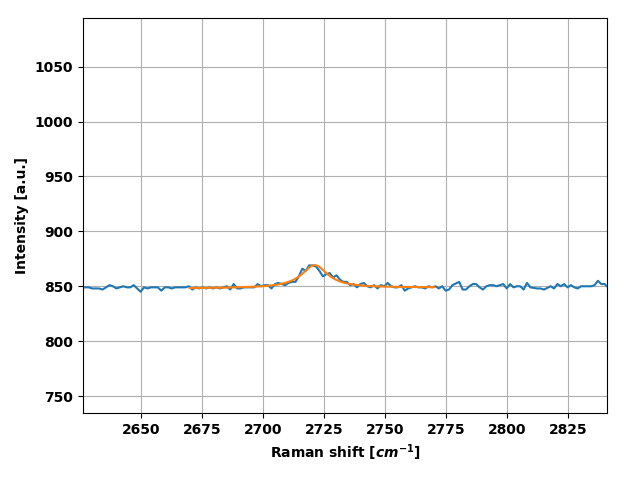
\includegraphics[scale=0.5]{Bilder/part6/prestine_2D.png}
\caption{Spectrum of pristine graphene measured with the blue laser and the same spectrum zoomed into the 2D-line. The G-line is not visible and the 2D-line has a very small intensity. The 2D-line position is $\omega_{2D} = \SI{2721.1(4)}{cm^{-1}}$.}
\label{fig:pristine}
\end{figure}

\begin{figure}
\centering
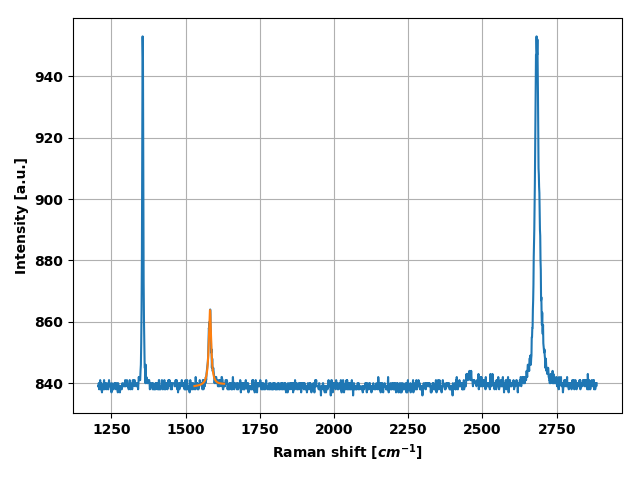
\includegraphics[scale=0.5]{Bilder/part6/prestine_green.png}
\caption{Spectrum of pristine graphene measured with the green laser in order to determine the position of the G-line. The G-line is highlighted and determined with $\omega_{G} = \SI{1582.4(3)}{cm^{-1}}$.}
\label{fig:pristine_green}
\end{figure}

\begin{figure}
\centering
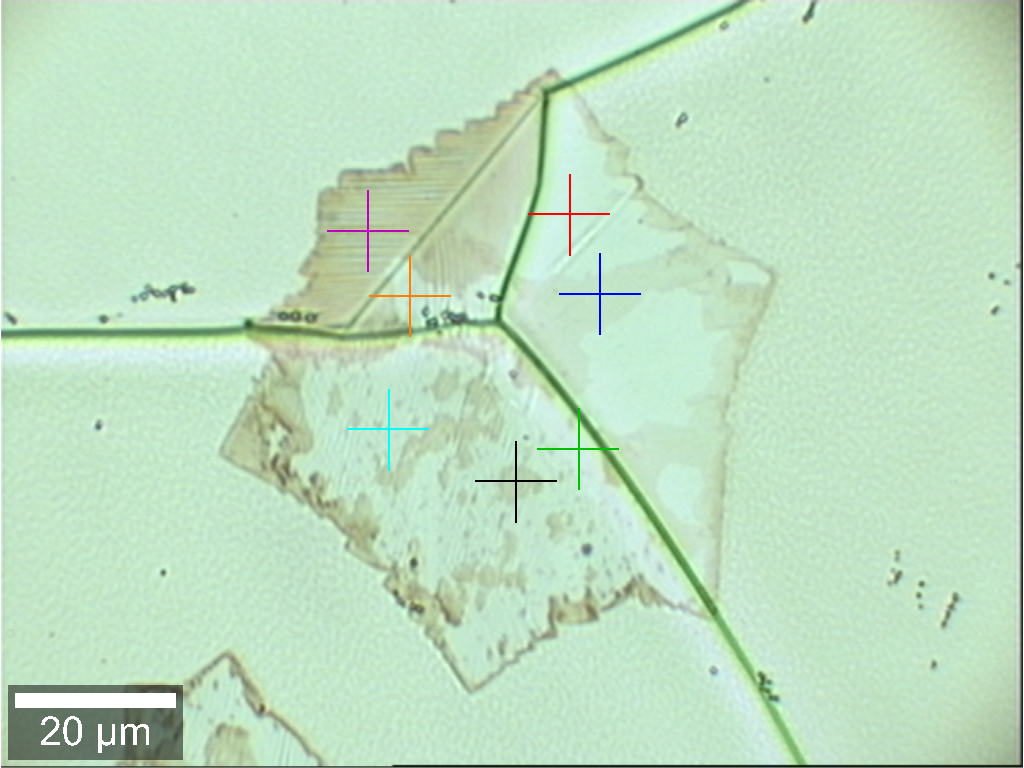
\includegraphics[scale=0.3]{Bilder/part6/4D4RamanFlake.png}
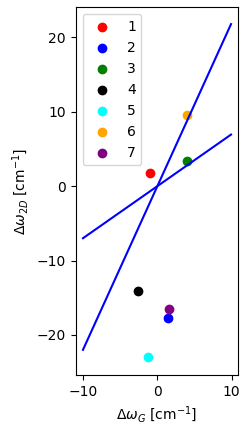
\includegraphics[scale=0.7]{Bilder/part6/map.png}
\caption{Left: Polycristalline sample. Measurement points in order of red, blue, green, black, cyan, orange, purple. Right: Map of the difference between the extracted line-positions and the pristine position.}
\label{fig:poly_sample}
\end{figure}


\begin{table}[h]
\centering
\begin{tabular}{|c|c|c|c|}
\hline 
Measurement & Miller indices & $\omega _G$ &  $\omega _{2D}$\\ 
point &  &  & \\ 
\hline 
pristine &  &\SI{1582.4(3)}{\per cm} & \SI{2721.1(4)}{\per cm}\\ 
\hline 
1(red) & (0.14,0.51,0.85) &\SI{1581.4 \pm 0.3}{\per cm} & \SI{2719.4 \pm 0.2}{\per cm}\\ 

\hline 
2(blue) & (0.14,0.51,0.85) & \SI{1583.8 \pm 0.2}{\per cm} & \SI{2701.7 \pm 0.2}{\per cm}\\ 
\hline 
3(green) & (0.33,0.56,0.76) & \SI{1586.4 \pm 0.2}{\per cm} & \SI{2722.8 \pm 0.5}{\per cm}\\ 
\hline 
4(black) & (0.33,0.56,0.76) & \SI{1579.8 \pm 0.2}{\per cm} & \SI{2705.3 \pm 0.4}{\per cm}\\ 
\hline 
5(cyan) & (0.33,0.56,0.76) & \SI{1581.1 \pm 0.3}{\per cm} & \SI{2696.4 \pm 0.5}{\per cm}\\ 
\hline 
6(orange) & (0.03,0.14,0.99) & \SI{1586.4 \pm 0.3}{\per cm} & \SI{2729.0 \pm 0.5}{\per cm}\\ 
\hline 
7(purple) & (0.03,0.14,0.99) & \SI{1583.9 \pm 0.2}{\per cm} & \SI{2702.9 \pm 0.3}{\per cm}\\ 
\hline 
\end{tabular} 
\caption{Results for the positions of G and 2D peak from the polycristalline sample at the measurement points as marked in Fig. \ref{fig:poly_sample}.}
\label{tab:part5_pos}
\end{table}

\begin{table}[h]
\centering
\begin{tabular}{|c|c|c|c|c|}
\hline 
Measurement &  Miller indices & Doping & uniaxial strain &  biaxial strain\\ 
point & & [$10^{-12} \si{cm^{-1}}$] & [\%] & [\%]\\ 
\hline
1 & (0.14,0.51,0.85) & $0.213 \pm 0.001$ & $-0.0503 \pm 0.0004$ & $-0.088 \pm 0.0007$ \\ 
\hline
2 & (0.14,0.51,0.85) & $6.044 \pm 0.009$ & $0.3914 \pm 0.0003$ & $0.6849 \pm 0.0005$ \\ 
\hline
3 & (0.33,0.56,0.76) &$0.408 \pm 0.001$ & $-0.0126 \pm 0.0004$ & $-0.022 \pm 0.0008$ \\ 
\hline
4 & (0.33,0.56,0.76) &$0.983 \pm 0.002$ & $0.2573 \pm 0.0004$ & $0.4503 \pm 0.0007$ \\ 
\hline
5 & (0.33,0.56,0.76) &$5.678 \pm 0.015$ & $0.4628 \pm 0.0005$ & $0.81 \pm 0.0010$ \\ 
\hline
6 & (0.03,0.14,0.99) &$0.009 \pm 0.001$ & $-0.1425 \pm 0.0005$ & $-0.2493 \pm 0.0009$ \\ 
\hline
7 & (0.03,0.14,0.99) &$5.488 \pm 0.009$ & $0.3677 \pm 0.0003$ & $0.6435 \pm 0.0006$ \\ 
\hline 
\end{tabular} 
\caption{Results for the positions of G and 2D peak from the polycristalline sample at the measurement points as marked in Fig. \ref{fig:poly_sample}.}
\label{tab:part5_results}
\end{table}

\section{Continuous Graphene}
The sample of continuous graphene on oxidized copper and the measured points are shown in figure \ref{fig:part7_sample}. In this chapter we want to analyze the defect density of the sample. Defects lead to the formation of different peaks, because the Raman process can involve defect scattering. In order to be able to analyze this the Intensity of the G-line and the D-line, which involves defect scattering, are determined. Both lines are analyzed with the same method used in previous chapters. The spectrums and fits can be seen in figure \ref{fig:part7_spectrum}. The extracted positions and Intensities are listed in table \ref{tab:part7_results}. With the help of the Model from  Cancado et al.\cite{cancado} the average distance between defects $L_D$ can be determined:
\begin{equation}
\dfrac{I_D}{I_G} = C_A \dfrac{(r_A^2 - r_s^2)}{(r_A^2 - 2 r_s^2)} (e^{-\pi r_s^2/L_D^2} -e^{-\pi (r_A^2 - r_s^2)/L_D^2})
\end{equation}
$C_A = 160 * E_L^{-4}$ with the laser energy $E_L = \SI{2.33}{eV}$, $r_s = \SI{1}{nm}$, $r_A = \SI{3.1}{nm}$ are used.\\
This function and the Intensity ratios of the measurement points are shown in figure \ref{fig:part7_fit}. $L_D$ and its error are visually estimated. This results in a average distance of $L_D = \SI{24(1)}{nm}$ for point 1 and $L_D = \SI{70(1)}{nm}$ for point 2.

\begin{figure}
\centering
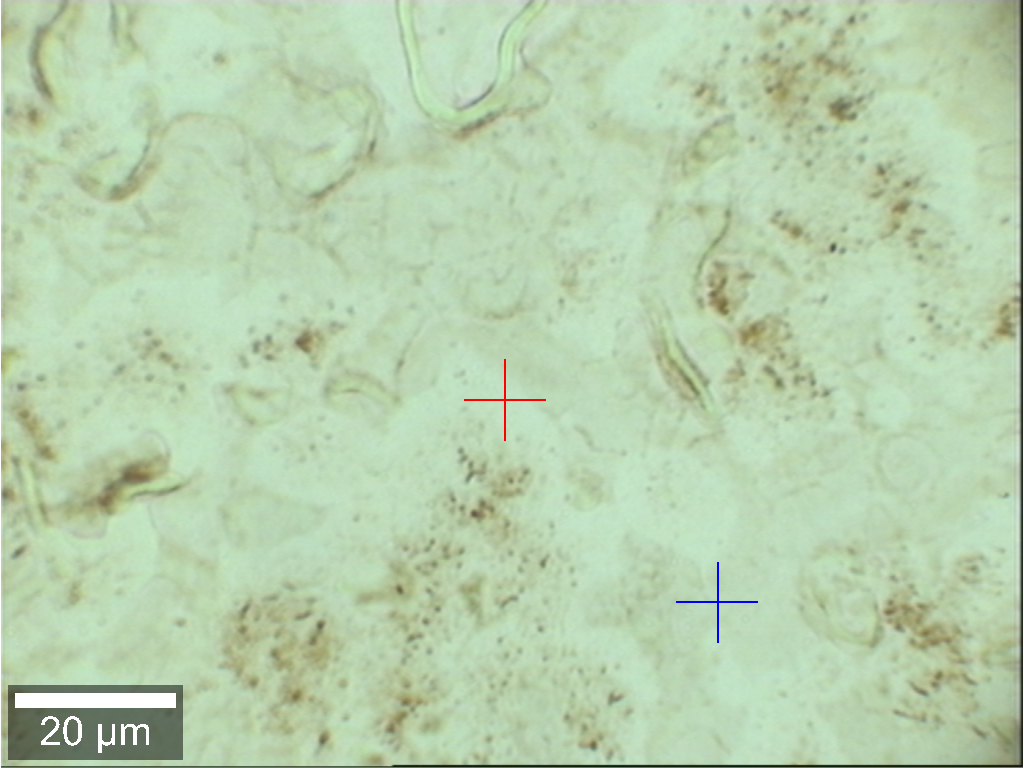
\includegraphics[scale=0.3]{Bilder/part7/Continuousoptical.png}
\caption{Left: Polycristalline sample. Measurement points in order of red, blue, green, black, cyan, orange, purple. Right: Map of the difference between the extracted line-positions and the pristine position.}
\label{fig:part7_sample}
\end{figure}

\begin{figure}
\centering
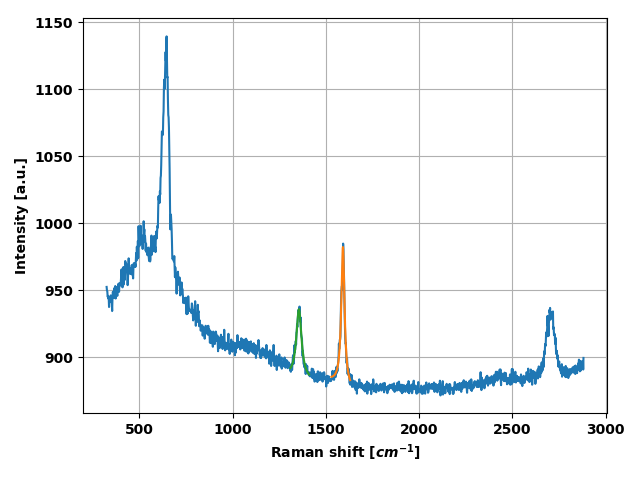
\includegraphics[scale=0.5]{Bilder/part7/1.png}
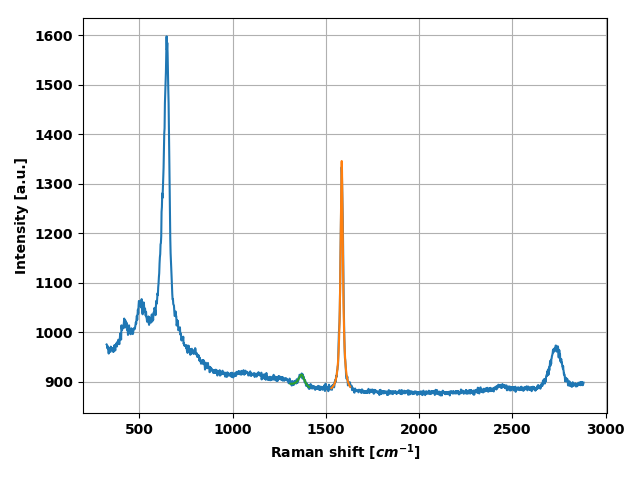
\includegraphics[scale=0.5]{Bilder/part7/2.png}
\caption{Extracted spectrums from the continuous graphene. Left: red point, right: blue point.}
\label{fig:part7_spectrum}
\end{figure}

\begin{table}
\centering
\begin{tabular}{|c|c|c|c|c|c|c|}
\hline 
Measurement &  $\omega_G[cm^{-1}]$  & $\omega_D[cm^{-1}]$& $I_G$ & $I_D$ & $I_D/I_G $ & $L_D[nm]$\\ 
point &  &  & & & &\\ 
\hline
1(red) & $1591.4 \pm 0.3$ & $1355.6 \pm 0.4$ & $103 \pm 2$ & $51 \pm 2$ & $0.50 \pm 0.02$ & $24\pm 1$\\ 
\hline
2(blue) & $1585.0 \pm 0.2$ & $1369.9 \pm 0.9$ & $468 \pm 2$ & $26 \pm 2$ & $0.06 \pm 0.01$ & $70\pm 1$\\ 
\hline
\end{tabular} 
\caption{Results for the positions of G and 2D peak from the polycrystalline sample at the measurement points as marked in Fig. \ref{fig:poly_sample}.}
\label{tab:part7_results}
\end{table}

\begin{figure}
\centering
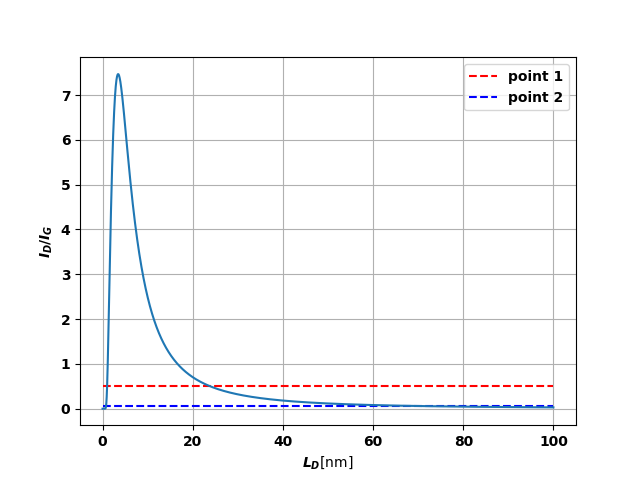
\includegraphics[scale=0.7]{Bilder/part7/fit.png}
\caption{Extracted spectrums from the continuous graphene. Left: red point, right: blue point.}
\label{fig:part7_fit}
\end{figure}


\section{Appendix}
\begin{figure}
\centering
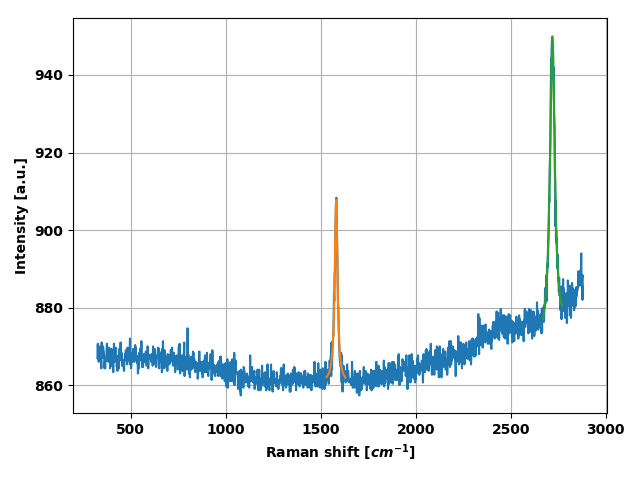
\includegraphics[scale=0.5]{Bilder/part6/1.png}
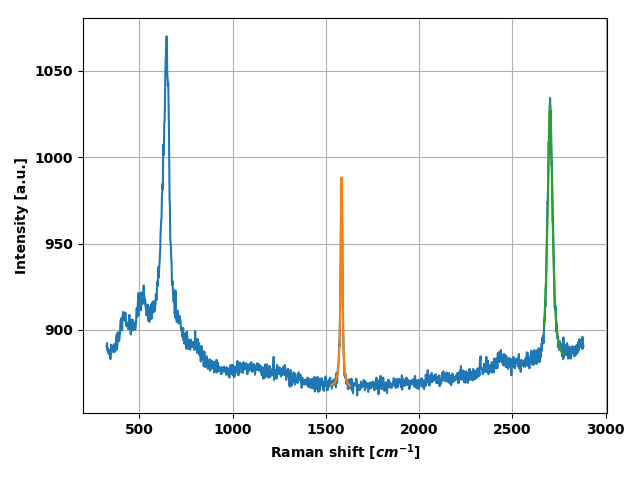
\includegraphics[scale=0.5]{Bilder/part6/2.png}
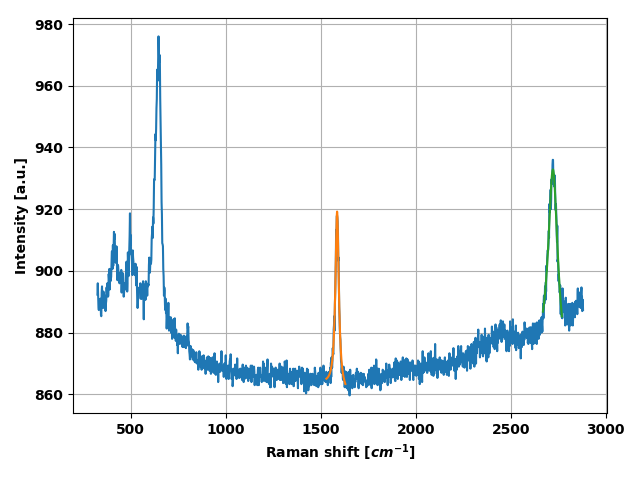
\includegraphics[scale=0.5]{Bilder/part6/3.png}
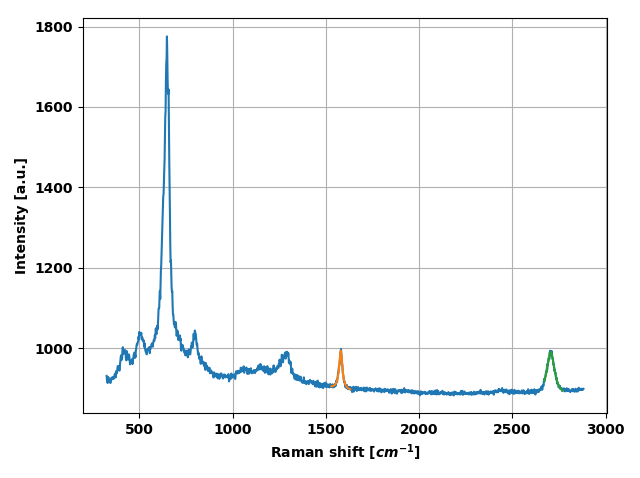
\includegraphics[scale=0.5]{Bilder/part6/4.png}
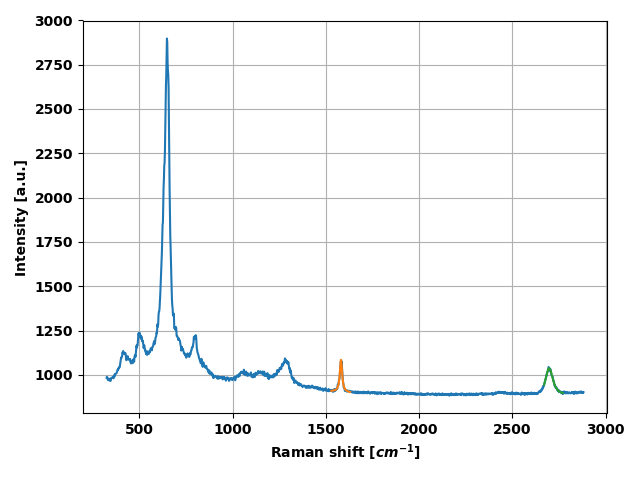
\includegraphics[scale=0.5]{Bilder/part6/5.png}
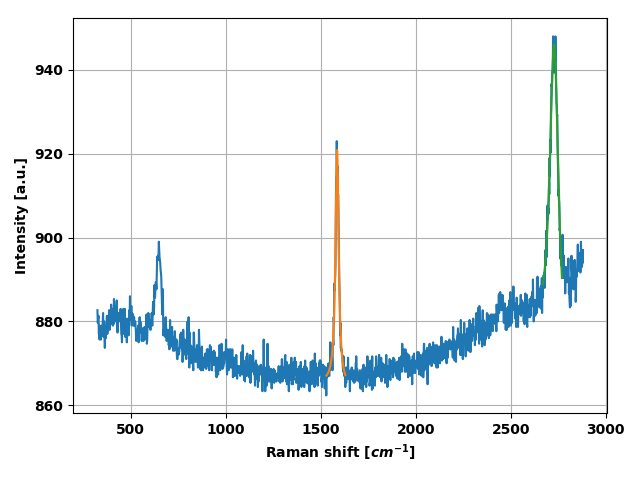
\includegraphics[scale=0.5]{Bilder/part6/6.png}
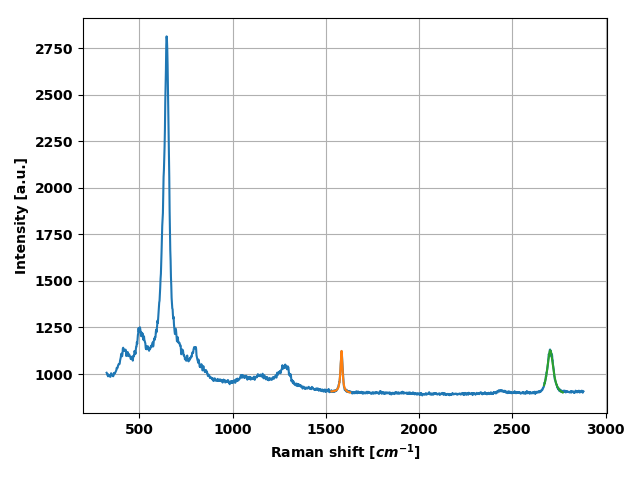
\includegraphics[scale=0.5]{Bilder/part6/7.png}
\caption{Spectra of the sample on polycristalline Cu. Top left is Measurement point 1 and bottom right point 7. The fits to the G and 2D-line are included.}
\label{fig:appendix_6}
\end{figure}



\bibliography{Ramanmo}

\end{document}